
\documentclass[11pt,a4paper,oneside]{book}
% \usepackage{a4wide}                     % Iets meer tekst op een bladzijde
\usepackage[dutch]{babel}               % Voor nederlandstalige hyphenatie (woordsplitsing)
\usepackage{amsmath}                    % Uitgebreide wiskundige mogelijkheden
\usepackage{amssymb}                    % Voor speciale symbolen zoals de verzameling Z, R...
\usepackage{makeidx}                    % Om een index te maken
\usepackage{url}                        % Om url's te verwerken
\usepackage{graphicx}                   % Om figuren te kunnen verwerken
\usepackage[small,bf,hang]{caption}     % Om de captions wat te verbeteren
\usepackage{xspace}                     % Magische spaties na een commando
\usepackage[latin1]{inputenc}           % Om niet ascii karakters rechtstreeks te kunnen typen
\usepackage{float}                      % Om nieuwe float environments aan te maken. Ook optie H!
\usepackage{flafter}                    % Opdat floats niet zouden voorsteken
\usepackage{listings}                   % Voor het weergeven van letterlijke text en codelistings
\usepackage[round]{natbib}              % Voor auteur-jaar citaties.
% \usepackage[nottoc]{tocbibind}		% Bibliografie en inhoudsopgave in ToC; zie tocbibind.dvi
\usepackage{eurosym}                    % om het euro symbool te krijgen
\usepackage{textcomp}                   % Voor onder andere graden celsius
\usepackage{fancyhdr}                   % Voor fancy headers en footers
% \usepackage[Gray,squaren,thinqspace,thinspace]{SIunits} % Om elegant eenheden te zetten
% \usepackage[version=3]{mhchem}          % Voor elegante scheikundige formules

% Volgend package is niet echt nodig. Het laat echter toe om gemakkelijk elektronisch
% te navigeren in je pdf-document. Deze package moet altijd als laatste ingeladen worden.
\usepackage[a4paper,plainpages=false]{hyperref}    % Om hyperlinks te hebben in het pdfdocument.


%%%%%%%%%%%%%%%%%%%%%%%%%%%%%%
% Algemene instellingen van het document.
%%%%%%%%%%%%%%%%%%%%%%%%%%%%%%

% De splitsingsuitzonderingen
\hyphenation{back-slash split-sings-uit-zon-de-ring}

%\bibpunct{(}{)}{;}{y}{,}{,}             % Auteur-jaar citaties -- zie natbib.dvi voor meer uitleg; niet echt nodig

% Het bibliografisch opmaak bestand.
% ZORG ERVOOR DAT bibliodutch.bst ZICH IN JE WERKDIRECTORY BEVINDT!!!
\bibliographystyle{bibliodutch}

\setlength{\parindent}{0cm}             % Inspringen van eerste lijn van paragrafen is niet gewenst.

\renewcommand{\baselinestretch}{1.2} 	% De interlinie afstand wat vergroten.

\graphicspath{{figuren/}}               % De plaars waar latex zijn figuren gaat halen.

\makeindex                              % Om een index te genereren.

\setcounter{MaxMatrixCols}{20}          % Max 20 kolommen in een matrix

% De headers die verschijnen bovenaan de bladzijden, herdefinieren:
\pagestyle{fancy}                       % Om aan te geven welke bladzijde stijl we gebruiken.
\fancyhf{}                              % Resetten van al de fancy settings.
\renewcommand{\headrulewidth}{0pt}      % Geen lijn onder de header. Zet dit op 0.4pt voor een mooie lijn.
\fancyhf[HL]{\nouppercase{\textit{\leftmark}}} % Links in de header zetten we de leftmark,
\fancyhead[HR]{\thepage}                % Rechts in de header het paginanummer.
% Activeer de volgende lijn en desactiveer de vorige om paginanummers onderaan gecentreerd te krijgen.
%\fancyhf[FC]{\thepage}                  % Paginanummers onderaan gecentreerd.

% PDF specifieke opties, niet strict noodzakelijk voor een thesis.
% Is hetgeen verschijnt wanneer je in acroread de documentproperties bekijkt.
\hypersetup{
    pdfauthor = {Gaspard Lequeux},
    pdftitle = {Een Introductie tot het Zetsysteem LaTeX},
    pdfsubject = {Cursus LaTeX opgebouwd als typevoorbeeld voor het schrijven van een thesis.},
    pdfkeywords = {LaTeX, zetsysteem, thesis, eindwerk}
}


% Het volgende commando zou ervoor moeten zorgen dat er een witte ruimte wordt gelaten tussen
% elke paragraaf. Het zorgt ervoor dat er echter teveel witte ruimte komt boven en onder de
% verschillende titels, gemaakt met \section, subsection...
%%\setlength{\parskip}{0ex plus 0.3ex minus 0.3ex}

% Vandaar dat we expliciet aangeven wanneer we wensen dat een nieuwe paragraaf begint:
% \par zorgt ervoor dat er een nieuwe paragraaf begint en
% \vspace zorgt voor vertikale ruimte.
\newcommand{\npar}{\par \vspace{2.3ex plus 0.3ex minus 0.3ex}}

%%%%%%%%%%%%%%%%%%%%%%%%%%%%%%
% Nieuwe commando's
%%%%%%%%%%%%%%%%%%%%%%%%%%%%%%

% De differentiaal operator
\newcommand{\diff}{\ensuremath{\mathrm{d}}} 

% Super en subscript
\newcommand{\supsc}[1]{\ensuremath{^{\text{#1}}}}   % Superscript in tekst
\newcommand{\subsc}[1]{\ensuremath{_{\text{#1}}}}   % Subscript in tekst

% Chemische formule font:
\newcommand{\ch}[1]{\ensuremath{\mathrm{#1}}\xspace}	 
% Chemische pijl naar rechts:
\newcommand{\chpijlr}{\ensuremath{\hspace{1em}\longrightarrow\hspace{1em}}}
% Chemische pijl naar links:
\newcommand{\chpijll}{\ensuremath{\hspace{1em}\longleftarrow\hspace{1em}}}
% Chemische pijl naar links en rechts:
\newcommand{\chpijllr}{\ensuremath{\hspace{1em}\longleftrightarrow\hspace{1em}}}

\newcommand{\vt}[1]{\ensuremath{\boldsymbol{#1}}} % vector in juiste lettertype
\newcommand{\mx}[1]{\ensuremath{\mathsf{#1}}}	  % matrix in juiste lettertype

% Het latex logo in een eenvoudiger commando steken
\newcommand{\latex}{\LaTeX\xspace}

% Het BibTeX logo
\newcommand{\bibtex}{\textsc{Bib}\TeX\xspace}

% Niew commando om bestandnamen anders weer te geven
\newcommand{\bestand}[1]{\lstinline[basicstyle=\sl]{#1}\xspace}

% Niew commando om commando tekst weer te geven
\newcommand{\command}[1]{\lstinline[basicstyle=\tt]{#1}\xspace}
\newcommand{\commandx}[1]{\index{#1}\lstinline[basicstyle=\tt]{#1}\xspace}

%\lstset{morecomment={\%}}
% Commando om latex commando`s weer te geven (x: voor indexing)
%\newcommand{\lcommand}[1]{\lstinline[basicstyle={\tt},{language=[LaTeX]TeX}]{#1}\xspace}
\newcommand{\lcommand}[1]{\lstinline[basicstyle={\tt}]{#1}\xspace}
\newcommand{\lcommandx}[1]{\index{#1}\lstinline[basicstyle=\tt]{#1}\xspace}


% Niew commando om vreemde taal weer te geven (hint: dit commando kan gebruikt
%   worden om latijnse namen, die ook cursief moeten staan, weer te geven.
\newcommand{\engels}[1]{\textit{#1}\xspace}
\newcommand{\engelsx}[1]{\index{#1}\textit{#1}\xspace}

% Niew commando om iets te benadrukken en tegelijkertijd in de index te steken.
\newcommand{\begrip}[1]{\index{#1}\textbf{#1}\xspace}

% Nieuw commando om figuren in te voegen. Gebruik:
% \mijnfiguur[H]{width=5cm}{bestandsnaam}{Het bijschrift bij deze figuur}
\newcommand{\mijnfiguur}[4][ht]{            % Het eerste argument is standaar `ht'.
    \begin{figure}[#1]                      % Beginnen van de figure omgeving
        \begin{center}                      % Beginnen van de center omgeving
            \includegraphics[#2]{#3}        % Het eigenlijk invoegen van de figuur (2: opties, 3: bestandsnaam)
            \caption{#4\label{#3}}          % Het bijschrift (argument 4) en het label (argument 3)
        \end{center}
    \end{figure}
    }

% Nieuw commando om figuren in te voegen. Gebruik:
% \mijnfiguur[H]{bestand-tabular}{Het bijschrift bij deze tabel}    
\newcommand{\mijntabel}[3][ht]{             % Het eerste argument is standaar `ht'.
    \begin{table}[#1]                       % Beginnen van de table omgeving
        \begin{center}                      % Beginnen van de center omgeving
            \caption{#3\label{#2}}          % Het bijschrift (argument 3) en het label (argument 2)
            \input{#2}                      % Invoer van de tabel
        \end{center}
    \end{table}
    }

%%%%%%%%%%%%%%%%%%%%%%%%%%%%%%
% Nieuwe wiskunde operatoren
%%%%%%%%%%%%%%%%%%%%%%%%%%%%%%

\DeclareMathOperator{\integ}{Integraal}

%%%%%%%%%%%%%%%%%%%%%%%%%%%%%%
% Nieuwe omgevingen
%%%%%%%%%%%%%%%%%%%%%%%%%%%%%%

% Een soort theorem omgeving
\newtheorem{levensles}{Levensles}[chapter]

% Om minder belangrijke delen iets kleiner te zetten.
\newenvironment{MinderBelangrijk}{\small}{}

% Een nieuwe omgeving om letterlijke latex tekst weer te geven.
\lstnewenvironment{llt} 
    {
    \vspace{1.2ex plus 0.5ex minus 0.5ex}   % Beetje ruimte voor de letterlijke tekst
    \lstset{                                % Enkele opties:
        basicstyle={\small\tt},             % Iets kleiner
        %language=[LaTeX]{TeX},              % Syntax highlighting
        stepnumber=0,                       % De lijnen worden niet genummerd
        breaklines=true,                    % Als een lijn te lang is, wordt hij afgebroken
        basewidth={0.5em},                  % Breedte van een letter
        xleftmargin=1em}                    % Inspringing van de linker marge
    }
    {\vspace{0.9ex plus 0.5ex minus 0.5ex}  % Beetje ruimte na de letterlijke tekst
    }

% Een nieuwe omgeving om algemene letterlijke tekst weer te geven.
\lstnewenvironment{lt} 
    {
    \vspace{1.2ex plus 0.5ex minus 0.5ex}   % Beetje ruimte voor de letterlijke tekst
    \lstset{                                % Enkele opties:
        basicstyle={\small\tt},             % Iets kleiner en typmachine lettertype
        stepnumber=0,                       % De lijnen worden niet genummerd
        breaklines=true,                    % Als een lijn te lang is, wordt hij afgebroken
        basewidth={0.5em},                  % Breedte van een letter
        xleftmargin=1em}                    % Inspringing van de linker marge
    }
    {\vspace{0.9ex plus 0.5ex minus 0.5ex}  % Beetje ruimte na de letterlijke tekst
    }



%%%%%%%%%%%%%%%%%%%%%%%%%%%%%%
% Einde van de preamble.
% Begin van de body:
%%%%%%%%%%%%%%%%%%%%%%%%%%%%%%

\begin{document}

\frontmatter

%  Titelblad

\begin{titlepage}

\fontsize{12pt}{14pt}\selectfont

\begin{center}

% Het logo van de Universiteit Gent

\includegraphics[height=3cm]{figuren/ruglogo}

\vspace{1cm}

\fontsize{14pt}{17pt}\selectfont
% De Faculteit:
\textsc{Faculteit Industri\"ele wetenschappen Afstudeerrichting: Informatica}
\fontsize{12pt}{14pt}\selectfont
\vspace{0.3cm}

\vspace{1.2cm}

%Het academiejaar
Academiejaar 2015--2016

\vspace{2.8cm}

\fontsize{17.28pt}{21pt}\selectfont

% De titel van de thesis:
{\textsc{Uitbreidbare web-gebaseerde intermodale routeplanner voor Belgi�}}

\fontseries{m}
\fontsize{12pt}{14pt}\selectfont

\vspace{1cm}

% De auteur van de thesis:
Brecht \textsc{Van de Vyvere}	

\vspace{1cm}

% De promotors van de thesis:
Promotors:\\ Prof.~dr.~ir.~R.~Van de Walle\\ Prof.~dr.~ir.~E.~Mannens

\vspace{0.5cm}

% De begeleiders van de thesis:
Begeleiders:\\ ~dr.~ir.~R.~Verborgh\\ ~ing.~P.~Colpaert

\vspace{1cm}

% De functie van de thesis:
Masterproef voorgedragen tot het behalen van de graad van\\
\textsc{Industrieel ingenieur: informatica}

\end{center}
\end{titlepage}

\thispagestyle{empty}
                            % Algemene versie
%\input{lc-titel-boerenkot}                  % Versie 2de kan informatica bio-ir

\mbox{}\vspace{12cm}

{
\footnotesize
Copyright 2003, 2004, 2005, 2006, 2007, 2008 Gaspard Lequeux. 
Alle rechten voorbehouden.
Dit werk mag worden verveelvoudigd en/of openbaar gemaakt door middel van druk, fotokopie, microfilm, geluidsband, kleitabletten, elektronische of welke andere wijze ook, onder de volgende voorwaarden:

\begin{itemize}
\item Vermelding van de auteur.
\item Niet commercieel. Dit vloeit voort uit het feit dat sommige paragrafen overgenomen werden uit \citet{vanOostrum96}, wiens werk niet mag gebruikt worden voor commerci�le doeleinden.
\item Als je dit werk wijzigt en/of verdeelt, moet dit gebeuren onder dezelfde voorwaarden. %Uitgeverijen mogen dus dit werk verbeteren en in boekvorm uitbrengen, maar mogen het kopi�ren van dat boek niet verbieden. % Deze zin is fout: commercieel gebruik is niet toegelaten!!!
\end{itemize}
\npar
\npar
De auteur is niet aansprakelijk voor eventuele fouten en onvolledigheden in dit werk. 
\npar
\npar
Versie 0.6.0\\
Gecompileerd op: \today
}

%
% Typisch copyright voor een thesis.
% Te plaatsen juist na het titelblad.

\rule[-0.4\baselineskip]{0cm}{10\baselineskip}   
\par \vspace{2.3ex plus 0.3ex minus 0.3ex}
De auteur en promotor geven de toelating deze scriptie voor consultatie beschikbaar te stellen en delen ervan te kopi�ren voor persoonlijk gebruik. Elk ander gebruik valt onder de beperkingen van het auteursrecht, in het bijzonder met betrekking tot de verplichting uitdrukkelijk de bron te vermelden bij het aanhalen van resultaten uit deze scriptie.
\par \vspace{2.3ex plus 0.3ex minus 0.3ex}
The author and promoter give the permission to use this thesis for consultation and to copy parts of it for personal use. Every other use is subject to the copyright laws, more specifically the source must be extensively specified when using from this thesis.
\par \vspace{2.3ex plus 0.3ex minus 0.3ex}
Gent, Januari 2016 % Vul de juiste datum in!!!
\par \vspace{2.3ex plus 0.3ex minus 0.3ex}

De promotors \hfill De begeleiders \hfill De auteur
\npar
\vspace{2cm}
\npar
% Pas de volgende lijn aan!!!
Prof.~dr.~ir.~R.~Van de Walle \hfill dr.~ir.~R.~Verborgh \hfill Brecht Van de Vyvere
Prof.~dr.~ir.~E.~Mannens ing.~P.~Colpaert                                          

\thispagestyle{empty} 

                   % Voor een echte thesis.
\newpage
%\mbox{}\vspace{-1cm}
%\thispagestyle{plain}

%\textbf{\Huge{Woord vooraf}}

\chapter*{Woord vooraf}

%\vspace{2cm}

\begin{slshape}

%\small
Deze cursus werd in November 2003 voor het eerst uitgegeven in het kader van een Zeus (Studenten Werkgroep Informatica) initiatief om thesistudenten te helpen hun thesis in een aantrekkelijke vorm te gieten. De tekst is opgevat als een soort minithesis zodat studenten gemakkelijk alles kunnen overnemen. Om die reden zijn de bronbestanden beschikbaar gemaakt op het internet.\footnote{\url{http://zeus.ugent.be/~gaspard/latex}} 
\npar
Hoewel sommige deeltjes van deze cursus expliciet gericht zijn op het maken van een thesis, kan de tekst gebruikt worden als algemene inleiding op \latex. In 2004 zag ook Prof. Ottoy dit in. Vandaar dat deze cursus nu deel uitmaakt van de lessen informatica in de tweede bachelor bio-ir van de Universiteit Gent. Bij die gelegenheid heeft hij de cursus volledig nagekeken op taalfouten, waarvoor dank.
\npar
In 2006 heeft Prof. Dawyndt de cursus ook grondig herlezen en nagekeken, waarvoor dank. Sindsdien wordt deze cursus gebruikt in de lessen Computergebruik gegeven in de eerste bachelor Informatica van de Universiteit Gent.
\npar
Voor het schrijven van deze handleiding \latex, werd gebruik gemaakt van twee werken: \textsf{A guide to \latex} van \citet{kopka99} en \textsf{Handleiding \latex} van Piet van Oostrum (1996). Uit dit laatste werden zelfs hele paragrafen overgenomen. Daarnaast werd natuurlijk rijkelijk geput uit de documentatie die meegeleverd wordt met \latex zelf.
\npar
Minder belangrijke delen worden in een kleiner lettertype weergegeven. Verder zijn er verschillende voetnoten die verwijzen naar \latex documentatie op een Debian GNU/Linux systeem. Niemand gebruikt dat natuurlijk. Maar de bedoeling ervan is dat de lezer weet dat de documentatie bestaat, welke bestandsnaam die heeft en waar ongeveer die te vinden is in de \latex directorystructuur. Het is dan niet zo moeilijk meer om in je favoriete besturingssysteem te zoeken naar de desbetreffende bestandsnaam. 
\npar
In een standaard MikTeX installatie (d\'e \latex distributie voor Windows), zijn de helpfiles van de verschillende \latex packages te vinden in \bestand{C:\\texmf\\doc\\latex}. In \bestand{C:\\texmf\\doc\\guides} zijn enkele algemene handleidingen te vinden over \latex.
\npar
Het woord vooraf dient ook om mensen te bedanken: 

\begin{itemize}

\item De mensen van Zeus, voor de stimulerende Vrije--\engels{Open Source} sfeer en het organiseren van lessen hier rond. 

\item Schamper, het studentenblad van de Universiteit Gent, voor het leveren van de promotor van dit werk.

\item Rudy Gevaert, die in het academiejaar 2001-2002 als eerste een \latex les gaf.

\item Geert Vernaeve, voor het eerste contact met \latex en het C-voorbeeld op bladzijde \pageref{cvoorbeeld}.

\item Mensen die fouten rapporteerden en/of verbeteringen suggereerden: David De Wolf, Annelies Huyck, Yves Nevelsteen, Stijn Gors, Geert Vernaeve, Michiel Meire, Hendrik Maryns, Olivier Verhoogen, Jean-Pierre Ottoy, Hugo Coolens, Lieven Clement, Andy Peene, Reinout Debergh, Frederik De Schrijver, David van der Ha, Brecht Donckels, Dominique Lebbe, Christopher De Dobbelaere, Paul Vogels, Heidi Vanparys, Stijn Depuydt, Veerle Gevaert, Joke Van Hevele, Katrien De Dauw, Francis Santens, Nicolas Vanden Bossche en Peter Dawyndt.

\item De (thesis)studenten van het Boerenkot,
%\footnote{Ook nog wel Faculteit Landbouwkundige en Toegepaste Biologische Wetenschappen genoemd, maar niemand gebruikt die lange naam ;-)}
die in 2003 gevraagd hebben naar deze handleiding.

\end{itemize}

\latex lijkt in het begin moeilijk: alles in tekstmode, geen knopjes, je moet speciale commando's kennen om iets te bereiken~\ldots\ De eerste dagen zul je inderdaad enkele problemen ondervinden. Zoeken, doorbijten en hulp vragen aan meer ervaren gebruikers zullen ervoor zorgen dat je na enkele weken zelfs je wiskundige redeneringen rechtstreeks in \latex uitvoert. 
\npar
Deze handleiding is waarschijnlijk niet fautloos. Het rapporteren van meer dan ��n fout, zorgt voor je naam in de volgende editie van dit woord vooraf. Ook inhoudelijke opmerkingen zijn steeds welkom.

\vspace{4ex}

\hfill Gaspard Lequeux

\hfill Gent 9 Augustus 2006

%\normalsize
\end{slshape}

                      % Algemene versie
%\input{lc-woordvooraf-boerenkot}            % Versie 2de kan informatica bio-ir

% Voor een echte thesis, komt hier de samenvatting...
%\input{samenvatting}                       % ...in het Nederlands en...
%\input{summary}                            % ...in het Engels.

% De lijnen van de inhoudsopgave iets dichter op elkaar, niet echt nodig voor de thesis, maar 
% voor dit werk kregen we anders een laatste bladzijde met 3 items op.
\renewcommand{\baselinestretch}{1.08} 	% De interlinie afstand wat vergroten.
\small\normalsize                       % Nodig om de baselinestretch goed te krijgen.
\tableofcontents
\renewcommand{\baselinestretch}{1.2} 	% De interlinie afstand wat vergroten.
\small\normalsize                       % Nodig om de baselinestretch goed te krijgen.

\mainmatter

% De verschillende hoofdstukken:

\chapter{Inleiding}

\section{Routeplanning}

\subsection{Heden}
Routeplanners worden ge�mplementeerd met een API (Application Programming Interface) die al het werk voor zich neemt. Als een cli�nt van plaats X naar Y wil dan berekent de server de korste of snelste weg en geeft het resultaat terug. Om extra features op te vragen, moet de cli�nt parameters meegeven die vermeld staan in de documentatie van de API. Er is dus een sterke koppeling tussen cli�nt en server. Dankzij de opkomst van open data kunnen veel meer features toegevoegd worden aan een routeplanner. Een gebruiker kan bijvoorbeeld kiezen om niet door een regio met een hoog criminaliteitscijfer te reizen. Doordat alleen de server intelligente beslissingen kan nemen, wordt het moeilijk voor de cli�nt om features toe te voegen.

\subsection{Vernieuwing}
Binnen deze masterproef bespreken we een alternatieve methode voor routeplanning. Deze methode maakt gebruik van gelinkte connecties.

Een connectie is simpelweg het vertrek en aankomst van een voertuig. Neem je bijvoorbeeld de trein van station A naar station C en de trein stopt ook in station B, dan bestaat jouw route uit twee connecties: die tussen A en B, B en C. Het kan dus ook zijn dat je moet overstappen in station B.

\begin{figure}[htbp]
   \centering
   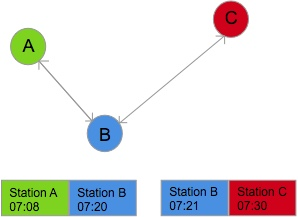
\includegraphics{connectionconcept.jpg} % requires the graphicx package
   \caption{Illustration of the route A - C that exists out of two connections.}
   \label{fig:example}
\end{figure}

Elke route die bestaat dus uit een combinatie van connecties die je via verschillende stations tot je bestemming brengen. 

Deze masterproef onderzoekt hoe connecties van verschillende transportmodi gecombineerd kunnen worden.

\subsection{Voor- en nadelen}
\begin{itemize}
\item Verschillende cli�nts kunnen gemakkelijk gemaakt worden. 
\item Algoritmes die rekening houden met verschillende contexten, bv. rolstoeltoegankelijkheid.
\item Interoperabiliteit van verschillende transitmodi is een Linked Data probleem. Hoe andere stops van andere transportmiddelen bereikbaar zijn, wordt later verduidelijkt. 
\item Schaalbaar: een vervoermaatschappij toevoegen maakt het zoeken van een optimale route niet complexer.
\item Performant dankzij caching.
\end{itemize}

\section{Hoe het begon}

\subsection{Open Data}
Mensen hebben nood aan gebruiksvriendelijke apps die correct gegevens tonen in de juiste context. Bij overheidsdiensten of bedrijven waar elke burger de zogenaamde klant is, ligt de rol van apps bouwen minder bij het de instantie zelf.
Meer en meer bedrijven en overheidsinstanties publiceren hun tijdstabellen als open data. Bij transportbedrijven, zoals De Lijn, is dit ook het geval.

\subsection{GTFS}
GTFS staat voor General Transit Feed Specification. Deze specificatie bepaalt hoe de data van de tijdstabellen van vervoersmaatschappijen opgesteld moet worden. Hierdoor ontstaan er interessante mogelijkheden voor routeplanning door deze GTFS feeds te kunnen combineren.



\chapter{Conclusies en perspectieven}

Elk goed werk eindigt met algemene slotconclusies (pleonasme) en een blik op wat beter kan (maar niet elk werk dat daarmee eindigt is een goed werk). Nu, bij deze cursus zijn er niet veel conclusies. Perspectieven zijn er des te meer. We hebben het vooral gehad over de syntax van \latex. Niet over de programma's er rond. Mensen die met \latex blijven werken, worden door de jaren heen zeer kritisch over de kwaliteit van hun documenten. Maar niet alleen hun documenten, heel hun (computer) tot op het pathologische af.\footnote{Waarom denk je, werd deze cursus geschreven op een Debian GNU/Linux systeem? Omdat dat gratis is? Nee! Omdat het beter is? Speelt vast en zeker mee. Maar de belangrijkste reden is de \textsc{Vrijheid} van dat systeem!} Bijgevolg zijn de programma's er rond zeer belangrijk.
\begin{itemize}
\item \command{make} Bij de finalisatie van een document, moeten verschillende commando's opgeroepen worden: 1 keer \command{latex}, 1 keer \command{bibtex}, 3 keer \command{latex}, 1 keer \command{makeindex}, 2 keer \command{latex}. Met een \bestand{Makefile} kan je dat allemaal inkorten tot ��n enkel commando: \command{make full}.
\item \command{ispell} Spellingscontrole.
\item \command{xfig} Voor maximale homogeniteit tussen de figuren en de tekst. De letters op je figuur zijn dezelfde als die in je document.
\item \command{vim} De teksteditor. In het begin moeilijk te gebruiken, maar ��n keer je er mee weg bent, lijken alle andere tekstverwerkers zo kleurloos.
\item \command{gimp} \engels{GNU Image Manipulation Program}. Om figuren op te poetsen.
\item \command{gnuplot}, \lcommand{grace} Voor het omzetten van data in grafieken.
\end{itemize}




% De appendices:
\appendix

% \input{lc-bijlage-mathsymbols}

% De bibliografie en de index
\backmatter

\bibliography{lc-bibliografie}

\printindex                             % Om de index af te printen, niet bij een thesis.

\end{document}

